 
\newpage
\setcounter{section}{37}
\section{Понятие рёберной двусвязности. Отношение эквивалентности.}

\textbf{Определение.} Две вершины реберно двусвязны, если между ними существуют два пути без общих ребер.
   
Нетрудно показать, что отношение реберной двусвязности является отношением эквивалентности. Действительно, рефлексивность и симметричность очевидны из определения.\\
\textbf{Докажем транзитивность $a \sim b, b \sim c \Rightarrow a \sim c$ :}

\begin{proof}
Рассмотрим два пути из $c$ в $b$. Найдём их места первого пересечения с циклом $a \to b \to a$, получили вершины $x$ и $y$. 
Тогда есть рёберно не пересекающиеся пути $a \to x \to c$, $a \to y \to c$. \\

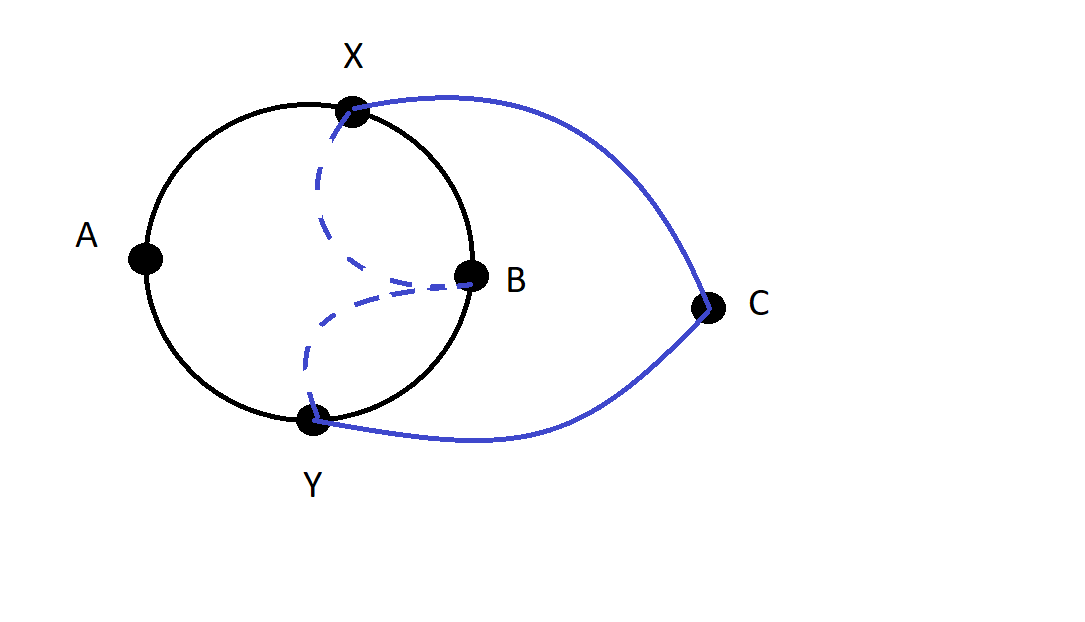
\includegraphics[width=0.5\textwidth]{images/38_1.png}
\end{proof}

В этом случае введем понятие ниже.
        
\textbf{Определение.} Компонентами рёберной двусвязности графа называют его подграфы, множества вершин которых~---  классы эквивалентности рёберной двусвязности, а множества рёбер~--- множества ребер из соответствующих классов эквивалентности.
        
\textbf{Определение.} Мост~--- ребро, при удалении которого число компонент связности увеличивается.

\setcounter{section}{38}
\section{Выделение компонент рёберной двусвязности в неориентированном графе. Древесность графа со сжатыми компонентами рёберной двусвязности.}

\begin{theorem}
Заметим, что если удалить из графа все мосты, то компоненты связности в полученном графе будут соответствовать компонентам реберной двусвязности в исходном.
\end{theorem}
\begin{proof}

1) Если на пути между какими-то двумя вершинами в исходном графе есть мост, то их придется отнести к разным компонентам реберной двусвязности (иначе между ними есть два пути без общих ребер, но тогда между ними есть путь, который не проходит через наш мост, а отсюда следует, что наш мост не является мостом).

2) Рассмотрим древесное ребро $(v;to)$. То есть такое, что в процессе обхода графа алгоритмом $dfs$ вершина $v$ является родителем вершины $to$ (в первый раз, когда мы увидели $to$). Если ребро $(v;to)$ не является мостом, то $v$ и $to$ реберно двусвязны.\\

Докажем это. Т.к. ребро не является мостом, то верно следующее неравенство: $ret[to] \leq tin[v]$. То есть мы можем прыгнуть из поддерева $to$ в $v$ или куда-то выше. Тогда между $v$ и $to$ есть два реберно непересекающихся пути. (Один -- $v \to to$, второй -- спустимся в поддерево $to$, совершим прыжок в $v$ или его предка, потом спустимся в $v$)

А, значит, все компоненты связности в полученном графе являются компонентами реберной двусвязности в исходном.
\end{proof}

Как следствие этой теоремы получаем эквивалентное определение моста:

\textbf{Определение.} Мост~--- ребро, соединяющее две компоненты реберной двусвязности.

\begin{theorem}
Если сжать все комоненты реберной двусвязности, то получится граф без циклов. А если граф изначально связен, то это дерево.
\end{theorem}
\begin{proof}
Пусть между компонентам реберной двусвязности есть простой цикл. Тогда можно построить и цикл, проходящий по вершинам исходного графа и содержащий ребра взятого нами цикла.

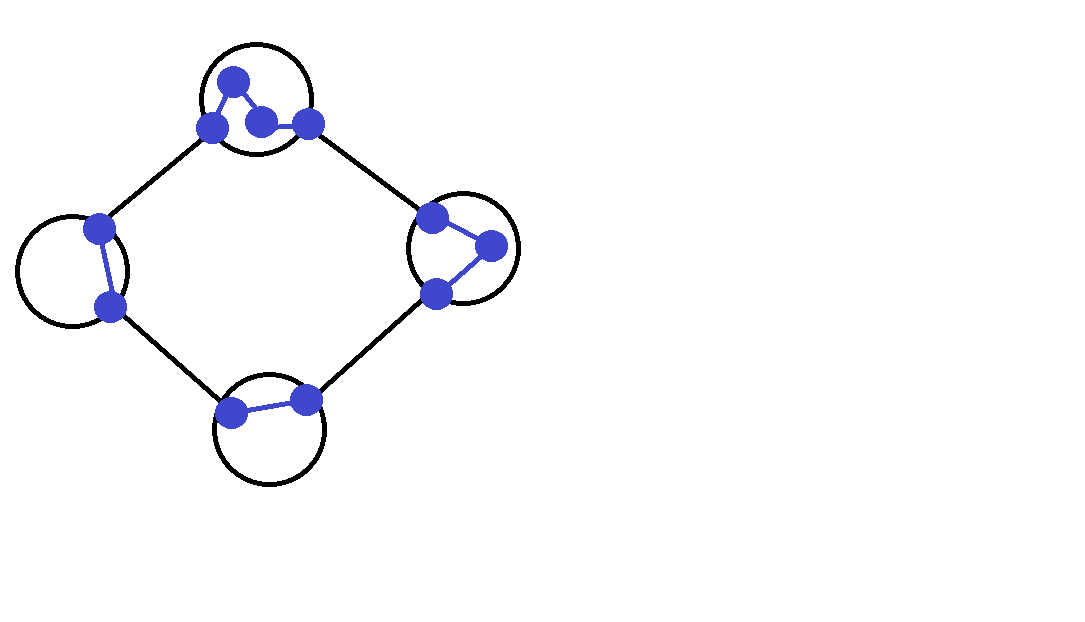
\includegraphics[width=0.5\textwidth]{images/39_1.png}

Но тогда все эти вершины лежат в одной компоненте реберной двусвязности. Получаем противоречие.
\end{proof}